%\bibliographystyle{sjtu2}%[此处用于每章都生产参考文献]
\chapter{动态场景下{\li}面临的挑战}
\label{chap:challenge}

尽管{\li}相比传统索引结构具有低空间消耗和短查询时间的优点。
然而,{\li}假设工作场景是只读的,即被索引的数据是固定不变,因此不需要处理更新操作,{\li}只需要一次构建即可长期使用,并假设访问是均匀分布的,
即所有数据被访问的概率是相同的,因此{\li}算法以优化所有键的访问平均时间为目标。

这样的假设极大地限制了{\li}地应用范围。
在真实场景下,伴随着写操作的执行,索引数据是频繁变化的,因此{\li}构建后面对持续变化的数据分布需要持续地进行架构调整以及训练来维持良好的{\li}性能。
同时,真实场景下工作负载是具有访问模式的,从而带来数据访问偏向性,即数据存在冷热之分,大量数据访问发生在少量的热点数据上,因此针对所有的键的平均访问时间进行优化是一种过度的优化目标,
并且以此作为优化目标的算法给{\li}带来性能上的缺陷。

面对广泛存在于真实场景里的动态场景,{\li}的现实应用存在许多挑战与机遇。
本节将探索并分析{\li}在动态场景下所面临的挑战。

\section{动态数据分布的挑战}
\label{sec:dist-challenge}

在真实场景下,伴随着写操作的执行,索引数据是频繁变化的,从而导致数据分布的动态变化,而{\li}的设计与测试中均为考虑静态的数据分布下的性能表现。
本小节将探动态数据分布、动态数据分布下{\li}的性能表现,并研究分析{\li}在动态数据分布下的所遇到性能问题的成因。

\subsection{动态数据分布}

在{\li}的语境下,数据分布包含两方面需要我们关注的指标{------}{\cdf}以及数据量大小。
{\cdf}的“形状”将决定{\rmi}中{\model}的拟合结果。
对于越“简单”的{\cdf},{\rmi}往往能够通过简单的{\model},比如{\lr},获得较好的精确度。
而数据量大小则更多影响{\rmi}最后级{\model}的个数,越多的数据量,往往需要更多的{\rmi}最后级{\model}来获得较好的性能。
除此之外,实际情况中在{\cdf}的“形状”与数据量大小均为发生变化时,如果搜索键的范围发生了移动,{\li}也需要通过重新训练来适应新的{\cdf}。

真实场景中存在这大量的写操作,包括插入、删除以及更新,其中更新操作可以看作是先删除再插入的组合操作。
因为写操作的存在,被索引的数据将持续地发生变化,从而影响{\cdf}与数量大小,导致真实场景下数据分布往往是动态变化的。
在真实场景下,几乎不存在静态的数据分布。
即使是以更新操作极为稀少的在线事务分析(on-line analytical processing,OLAP)也往往包括定期的数据更新操作,从而导致数据分布的变化。

\subsubsection{真实场景中的动态数据分布}

动态数据分布广泛地存在于真实的应用场景中,任何包含写操作的真实场景下数据分布都是动态的。
比如在电子商务应用中,添加商品信息、用户订单等操作,会不断地修改被索引的数据,从而导致数据分布的动态变化。

接下来我们通过{\tpcc}来展示广泛存在于真实场景中的动态数据分布。
{\tpcc}是一个用于测试事务处理系统性能与性价比的一个基准测试程序,被广泛地用来测试与评估商业数据库系统与数据库系统学术原型。
{\tpcc}是一个根据实际生产环境应用和环境而建模的在线事务处理(on-line transaction processing,OLTP)的基准测试程序。
作为一个在线事务处理基准测试程序,{\tpcc}模拟一个由终端操作员对于数据库执行交易的完整环境。
这个基准测试程序的中心是一个在订单输入的环境里的重要操作。
这些事务包括输入订单、运输订单、记录付款操作、检查订单状态以及统计仓库库存状态。

% The Transaction Processing Performance Council (TPC) is about to approve the third in its series of benchmarks which measure the performance and price/performance of transaction processing systems.
% Like TPC-A, the TPC's first benchmark, the new TPC Benchmark C, or TPC-C, is an on-line transaction processing (OLTP) benchmark.
% TPC benchmarks also differ from other benchmarks in that TPC benchmarks are modeled after actual production applications and environments rather than stand-alone computer tests which may not evaluate key performance factors like user interface, communications, disk I/Os, data storage, and backup and recovery.
% As an OLTP system benchmark, TPC-C simulates a complete environment where a population of terminal operators executes transactions against a database.
% The benchmark is centered around the principal activities (transactions) of an order-entry environment.
% These transactions include entering and delivering orders, recording payments, checking the status of orders, and monitoring the level of stock at the warehouses.
% However, it should be stressed that it is not the intent of TPC-C to specify how to best implement an Order-Entry system.
% While the benchmark portrays the activity of a wholesale supplier, TPC-C is not limited to the activity of any particular business segment, but, rather, represents any industry that must manage, sell, or distribute a product or service.

在{\tpcc}中,存在大量包含写操作的事务。
以新订单(New Order)事务为例,该事务执行过程中将向数据库输入一个完整的订单。
它代表了一个中等重量级、读写混合的事务,频繁被执行并且为了满足在线用户体验有着严格的反应时间的要求。
这个事务是{\tpcc}的核心事务。
新订单事务执行中,它在给定仓库、区域的组合下插入新的订单,并将该订单包含的商品一并插入数据库。
另一个代表性的事务是投递(Delivery)事务,这个事务会一次性处理10个尚未被投递的订单。
每个订单会在一个读写事务中被处理完成。
投递事务包含多个数据库事务,被执行的频率较低,对响应时间的要求更低。
通过不断执行新订单事务与投递事务,新订单表等相关数据库表被不断写入与删除订单对应的数据条目,从而使得相关表被不断地更新,而索引所面对的数据分布变得动态。

% The New-Order business transaction consists of entering a complete order through a single database transaction .
% It represents a mid-weight, read-write transaction with a high frequency of execution and stringent response time requirements to satisfy on-line users.
% This transaction is the backbone of the workload.
% It is designed to place a variable load on the system to reflect on-line database activity as typically found in production environments.

% The Delivery business transaction consists of processing a batch of 10 new (not yet delivered) orders.
% Each order is processed (delivered) in full within the scope of a read -write database transaction.
% The number of orders delivered as a group (or batched) within the same database transaction is implementation specific.
% The business transaction, comprised of one or more (up to 10) database transactions, has a low frequency of execution and must complete within a relaxed response time requirement.

\subsubsection{动态数据分布对通用索引结构性能的影响}

对于通用索引结构而言,动态数据分布下的读操作与写操作的复杂度往往没有本质上的区别。
以B树为例,它的读操作与写操作的复杂度都是$O(log(n))$,其中$n$为数据量大小。
然而,因为这些索引结构往往把数据结构完整性(integrity)的维护工作分摊在了每一次修改操作中,如B数的节点分裂(split)与合并(merge)操作是在每次写操作完成后进行的,
所以通常来说对于通用索引结构而言,写操作会有略高的操作复杂读。
同时,出于对并发性(concurrency)的考虑,并发索引结构可能会使用乐观并发控制或锁机制等方案来保证数据结构的一致性(consistency),从而再次对写操作的开销带来更多的负担。

\subsection{动态数据分布对{\li}性能的影响}
\label{sec:dist-affect-li}

与常见索引结构不同的是,{\li}在设计中仅考虑了不现实的静态数据分布的场景,即{\li}并不支持更新操作,因此面对动态数据分布,
{\li}性能将收到多方面的挑战\footnote{当然,最重要的一个挑战是如何高效地支持更新操作。然而这一问题超出了本文探究的范围,
在接下来的讨论中我们假设对{\li}的写操作能被高效处理,并探讨在这一基础之上{\li}性能面对的挑战。}。

正如上文提到,{\cdf}的“形状”发生变化时,{\rmi}架构需要重新选择,因为在过去的{\cdf}下能够进行高效拟合的{\model}可能将会产生更大的误差,从而导致{\li}的性能降低。
类似的,过去针对较难精确拟合的{\cdf}设计的{\rmi}架构可能对于新的{\cdf}而言有许多不必要的计算,比如{\rmi}层数太多与{\model}太复杂,从而产生更坏的{\li}性能。
同样的,数据量由少变多时,原有的{\rmi}最后级{\model}可能已经无法在较大的数据量下保持优秀的准确度,这时候可能需要通过调整{\rmi}最后级{\model}的个数或者更改{\model}类型来维持{\li}性能的影响的。
类似的,当数据量由多变少,{\model}类型以及{\rmi}最后级{\model}个数可能也需要进行调整来持续为索引操作提供良好的性能。

然而,尽管直观上我们可以总结出以上动态数据分布对{\li}性能的影响,但是由于{\model}难以量化的预测性能,我们缺乏可靠的规则来控制{\rmi}架构。
事实上,在第一次构建{\li}时,我们也缺乏可靠的指导依据来指导应该使用什么样子的{\rmi}架构,我们之能通过类似网格搜索\cite{lavalle2004relationship, lerman1980fitting}(grid search)的方法在一定搜索范围内通过枚举的手段来完成。
当数据分布发生变化时,为了维持{\li}的优秀性能,我们仍需要不断进行枚举搜索来确定{\rmi}架构。

\subsection{动态数据分布下搜索最优{\li}架构}
\label{sec:search-best}

寻找最优{\li}架构代价非常昂贵,往往需要大量的时间与计算资源才能决定最好的{\li}架构。
比如说,使用简单的搜索技术,如网格搜索搜索,往往需要10到100倍的训练时间。
{\li}的多级架构使这一任务更加困难,因为不同的级可以有不一样的{\model}类型和不同的{\model}数量,这些特性会指数级地增加架构搜索空间,
从而影响寻找最优{\li}架构成为非常昂贵的一项任务。

% \textbf{Second, it is costly to find the best model architecture.} It is usually expensive to decide the learning model's architecture.
% For example, it can take up to 10-100X of the model training time with basic search techniques such as grid search \cite{becsey1968nonlinear, lavalle2004relationship, bergstra2011algorithms}.
% \li's stage-based design makes this task even harder, as a different stage can have a different type of models, which exponentially increases the architecture search space.
% \input{distdata}

\begin{figure}[!ht]
  \centering
  % 
\includegraphics[width=4cm]{example/sjtulogo.png}
  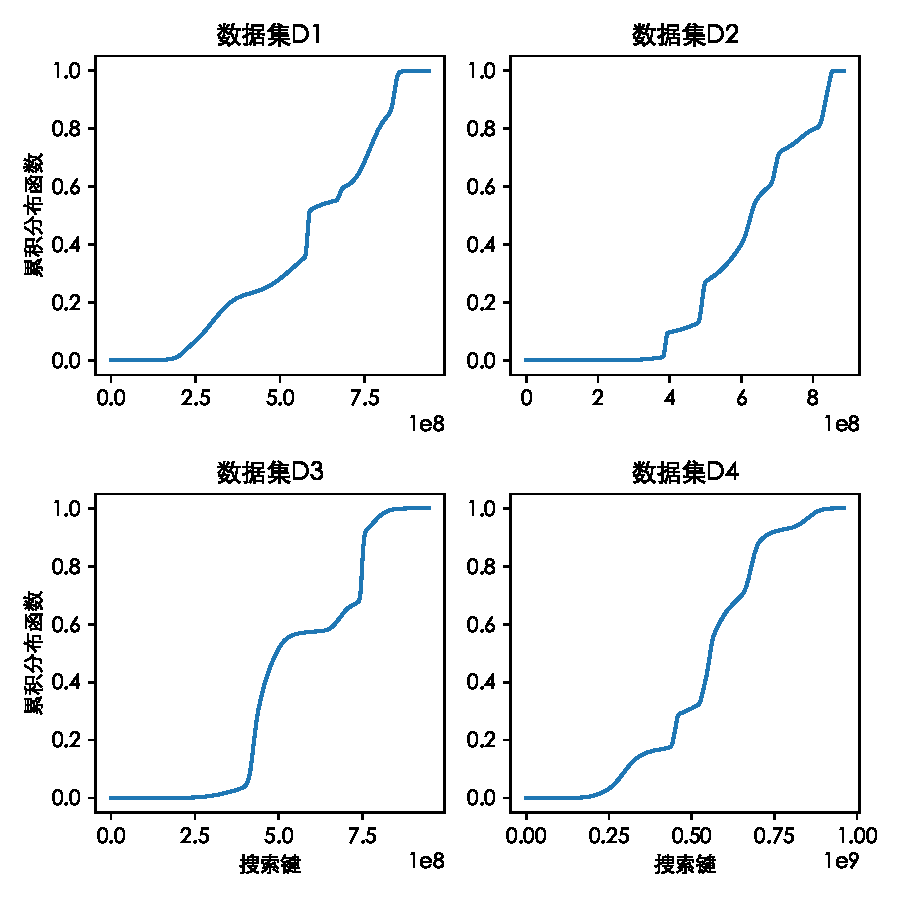
\includegraphics{figure/four-cdfs.pdf}
  \bicaption[不同数据集的{\cdf}]
    {不同数据集的{\cdf}}
    {CDFs of different datasets}
  \label{fig:dist}
\end{figure}

\begin{table}[!hpb]
  \centering
  \bicaption[不同数据集下使用第一级为{\nn}的{\rmi}架构的{\li}性能表现]
    % {一个颇为标准的三线表格\footnotemark[1]}
    {不同数据集下使用第一级为{\nn}的{\rmi}架构的{\li}性能表现}
    {The learned index performance with RMI architectures having neural netwrork at the first stage under different datasets}
  \label{tab:dist-nn}
  \begin{tabular}{lcccc}
    \toprule
                & \multicolumn{4}{c}{数据集}             \\ \cmidrule{2-5}
                & D1       & D2      & D3       & D4      \\ \midrule
    第一级{\nn}最优架构\footnotemark[1] & 1-12     & 1-8     & 1-12     & 1-16    \\
    吞吐量(MOPS)  & 2.08     & 2.11    & 2.13     & 2.07    \\
    损失函数        & 4.47e-4  & 7e-6    & 8.43e-4  & 1.5e-5  \\
    误差范围\footnotemark[2] & 7.86     & 7.39    & 7.56     & 7.48    \\ \bottomrule
  \end{tabular}
\end{table}
\footnotetext[1]{“$X$-$Y$”表示使用$X$个隐藏层、每个隐藏层包含$Y$个神经元的全联接神经网络。}

\begin{table}[!hpb]
  \centering
  \bicaption[不同数据集下使用第一级为{\lr}的{\rmi}架构的{\li}性能表现]
    % {一个颇为标准的三线表格\footnotemark[1]}
    {不同数据集下使用第一级为{\lr}的{\rmi}架构的{\li}性能表现}
    {The learned index performance with RMI architectures having linear model at the first stage under different datasets}
  \label{tab:dist-lr}
  \begin{tabular}{lcccc}
    \toprule
                & \multicolumn{4}{c}{数据集}              \\ \cmidrule{2-5}
                & D1       & D2      & D3       & D4       \\ \midrule
    吞吐量(MOPS)  & 2.24     & 2.01    & 1.89     & 2.28     \\
    损失函数  & 1.17e-3  & 2.79e-3 & 4.53e-3  & 8.91e-3  \\
    误差范围  & 7.84     & 8.50    & 9.20     & 7.91     \\ \bottomrule
  \end{tabular}
\end{table}

为了减少搜索空间,一个直观的启发式规则是“如果一个分布不能够被{\lr}较好地拟合,则应该使用更复杂的{\model},比如{\nn}”。
不幸的是,这一启发式规则并不能够其效果。
我们配置了四个不同分布的数据集(图\ref{fig:dist}),将{\li}架构限定为只有两级且第二级固定为1万个{\lr},并尝试用以上的启发式规则其决定第一级的{\model}类型。
在表\ref{tab:dist-nn}与表\ref{tab:dist-lr}中,当在第一级使用{\lr}时,它的损失函数{------}均方误差(mean square error)从第一个数据集(D1)到最后一个数据集(D4)不断增加。
这说明第一个数据集被{\lr}更好地拟合了,相比其他数据集。
同时,通过改变隐藏层(hidden layer)个数以及每个隐藏层的神经元(neuron)个数,我们尝试了不同{\nn}配置并选取了最优的{\nn}配置。
根据以上启发式规则,对于以上四个数据集,将第一级{\model}替换成{\nn}将会表现出越来越大的相对使用{\lr}的{\li}配置的性能提升。
然而{\nn}仅仅在第二个数据集(D2)和第三个数据集(D3)上提升了性能。

根据第\ref{sec:dist-affect-li}节的讨论,这一现象是符合预期。
这一现象之后有两个原因。
首先,{\nn}的计算代价远高于{\lr}{------}{\nn}需要80 ns而{\lr}仅需要16 ns,因此通过使用更复杂的{\model}来降低预测误差值需要支付更高的{\model}执行时间代价,
从而导致最终使用简单{\model}的{\rmi}配置会有更好的性能表现。
其次,尽管较高的损失函数值表示第一级的{\lr}的拟合结果不够精确,但这并不能够说明第二级的{\model}不能够很好地拟合数据。
因此,当在第一级使用{\lr}时,{\model}的平均误差值只比第一级使用{\nn}的架构稍微大一些。
因此,对于第四个数据集,最终具有更好性能的架构是使用{\lr}的架构。

% To reduce the search space, an intuitive heuristic is “if a distribution can not be fitted well with LR model, then we should use a complex model, like a neural netwrork (NN)”.
% Unfortunately, this heuristic does not work.
% We configure four datasets with different distributions, fix the second stage to have 10k LR models and try to use this heuristic to decide the first stage model type.
% \Cref{tab:distdata} shows that, when using LR as the first stage model, its loss (mean square error) increases from the 1st dataset (D1) to the last (D4).
% This means that D1 is much better fitted with LR than the others.
% Besides, we try different NN configurations with vary number of neural and depth and use the best.
% With the above heuristic, we should replace LR with NN of D2$\sim$D4.
% However, NN can only help to improve the performance for D2 and D3.
% There are two reasons make LR be better than NN for D4.
% First, NN's computation cost is much higher than LR ($\sim$80ns vs.
% 16ns); Second, even if the high loss value shows LR's fitting result is less accurate, but it does not indicate that the second stage models cannot fit the data well.
% As a result, when using LR as the first stage, the average error bound is only slightly worse than using NN.
% Thus, for D4, LR is the model should be used in the first stage.

出了这个启发式规则外,我们也尝试了目前最佳的优化方法{------}贝叶斯超参数优化(bayesian hyperparameter optimization){------}来寻找最优的{\li}架构成为非常昂贵的一项任务。
同样的,我们将搜索范围限定为只有两级且第二级固定为1万个{\lr},仅用这一方法来决定第一级的{\model}类型。
然而我们仍需要21分钟来找到最优的架构,这样的过长的搜索时间在真实场景下是不可接受的。

% Besides this heuristic, we also try to use some state-of-the-art technique~\cite{snoek2012practical}, bayesian hyperparameter optimization, to automatically search the best architecture.
% Even we constraint the stage number to be no larger than 2, it still takes about 21 minutes to find the best architecture.

\section{访问模式的挑战}

真实场景中数据访问往往不是均匀分布的,而是展现出不同的访问模式,而{\li}的设计与测试中均为考虑在不同的访问模式下的性能表现。
本小节将探讨何为访问模式、访问模式下{\li}的性能表现,并研究分析{\li}在变化各异的访问模式下的所遇到性能问题的成因。

\subsection{访问模式}

访问模式指的是一个系统或者程序对数据资源的读取或写入的模式。
这些模式在访问的局部性(locality of reference){------}在较短时间内对同一范围的数据资源重复地进行访问(读取与/或写入){------}水平上具有不同的体现。
有的访问模式具有较好的访问局部性,即在短时间内不断地读取或者写入同一范围的数据,而有的访问模式的访问局部性较差,即在该访问模式下大量的访问呈现出随机访问的特点,
每次访问的数据资源时间与空间上不具有较强的关联性。
前一种访问模式在各类计算机系统,包括文件系统、操作系统和数据库系统中较常出现,许多系统针对这一特点对在系统的设计与实现上进行了针对性的优化,从而提高系统的整体性能。
而后一种访问模式往往能够将系统的最坏性能展现出来,因为在这类访问模式之下,类似缓存等机制是无法有效缓解系统受较差访问局部性带来的性能影响的。

正如前文提到,访问模式对缓存机制的效用有较大影响,它还影响系统的并行与分布式计算的方式。
对于特定的访问模式,若将计算任务根据数据量或计算量进行简单的切割,并分散到多核或多机系统上进行执行,数据访问模式带来的竞争问题会极大地影响这种并行与分布式计算的性能提升。
由访问模式带来的在并行与分布式计算下的竞争问题中,最显而易见的就是因为一致性需求而导致的锁资源竞争,当大量的核或机器因为无法获取被竞争的锁时,系统将进入闲置状态,尽管仍然存在大量计算任务需要完成。

% In computing, a memory access pattern or IO access pattern is the pattern with which a system or program reads and writes memory on secondary storage.
% These patterns differ in the level of locality of reference and drastically affect cache performance,[1] and also have implications for the approach to parallelism[2][3] and distribution of workload in shared memory systems.
% [4] Further, cache coherency issues can affect multiprocessor performance,[5] which means that certain memory access patterns place a ceiling on parallelism (which manycore approaches seek to break[6]).

在数据库系统中,访问模式既包括对数据条目的访问模式,如是否存在在较短时间内的被频繁访问的数据条目或数据条目范围,也包括事务(transaction)执行的访问模式,
如是否存在在较短时间内的被频繁执行的事务以及事务是否以特定模式对数据条目进行操作。
这些访问最终都会涉及到对索引结构的访问,并转化成使用索引结构对键查找的访问模式。

综上所示,在本节的讨论中,我们仅考虑索引结构对键查找的访问模式所带来的挑战。
具体的,我们关注搜索键的访问局部性{------}在较短时间内对同一范围的搜索键是否有重复地进行访问(读取与/或写入)的特征。

\subsubsection{真实场景中的访问模式}

访问模式广泛地存在于真实的应用场景中。
比如对于电子商务应用,最新添加的数据,如商品信息、用户订单等,往往是最常被访问的,相反,
老数据很少被访问,比如多年前发生的交易信息等。

我们再次以{\tpcc}作为真实场景的样例。
在{\tpcc}中,存在大量具有特定访问模式的事务。
以新订单(New Order)事务为例,它在执行给定仓库、区域的组合下插入新的订单,并将该订单包含的商品一并插入数据库。
在{\tpcc}中,每个仓库、区域的组合具有独立的订单编号,并且该订单编号在每个仓库、区域的组合下是单增的。
因此,对于插入订单以及插入订单商品的操作,因为订单编号是作为对应表的主键之一,因此在插入过程中,对应表的主键索引总是被最大的订单编号进行索引操作。
新订单事务在{\tpcc}中占据了接近一般的执行次数,能否较好地处理这种访问模式将直接决定数据库能否高效地完成{\tpcc}以及{\tpcc}所建模代表地广泛的现实世界在线事务处理任务。

% The New-Order business transaction consists of entering a complete order through a single database transaction .
% It represents a mid-weight, read-write transaction with a high frequency of execution and stringent response time requirements to satisfy on-line users.
% This transaction is the backbone of the workload.
% It is designed to place a variable load on the system to reflect on-line database activity as typically found in production environments.

\subsubsection{访问模式对通用索引结构性能的影响}

对于大部分的索引结构,访问模式中的访问局部性特性均会对其性能产生不同程度的影响。
对于这些索引结构,具有较差的访问局部性或者不具有任何访问局部性,即纯粹的乱序访问,将展现出索引结构的平均性能,
因为不同的搜索键以接近随机的模式进行访问。
而当访问模式中具有较明显的访问局部性的时候时,往往能够利用计算机现有体系结构中的内存层级(memory hierarchy)的缓存机制获得一定的性能提升。
对于内存使用越少的索引结构,访问模式中较明显的访问局部性对索引性能的提升会更加明显。
但另一方面,如果不同的搜索键之间在索引结构中的性能有差异,比如说字典树及其变种的索引结构的索引操作性能与搜索键长度具有较强的关联性,
访问模式中较明显的访问局部性有可能反而会影响索引结构的操作性能,因为如果{\hotkey}恰好是性能较差的那一部分搜索键。

针对访问模式中潜在的访问局部性,相关索引结构研究就这一特点进行开发利用。
Huanchen等人提出混合索引\cite{zhang2016reducing},针对具有访问偏向性的动态场景进行优化。
混合索引通过冷热数据分离的方法。
第一级使用空间使用较少的、更新较灵活的热存储来处理写操作,这一部分的索引结构的尺寸较小以快速地响应读与写请求。
第二级用较为紧凑且只读的冷存储来存储大量的索引条目,这一部分的索引结构是针对读操作进行优化的,因为不需要支持实时更新操作,
所以许多针对写操作的设计可以被避免,从而获得较为紧凑的结构设计。
混合索引间接性地将第一级的索引条目从第一级迁移到第二级。
这样的混合索引结构在{\skewacc}下,能够有效地提供较好的空间利用率和高性能表现。

% The first stage ingests all incoming entries and is kept small for fast read and write operations.
% The index periodically migrates entries from the first stage to the second, which uses a more compact, read-optimized data structure.
% Our first contribution is hybrid index, a dual-stage index architecture that achieves both space efficiency and high performance.
% Our second contribution is Dual-Stage Transformation (DST), a set of guidelines for converting any order-preserving index structure into a hybrid index.
% Our third contribution is applying DST to four popular order-preserving index structures and evaluating them in both standalone microbenchmarks and a full in-memory DBMS using several transaction processing workloads.
% Our results show that hybrid indexes provide comparable throughput to the original ones while reducing the memory overhead by up to 70%.

\subsection{访问模式对{\li}性能的影响}
\label{sec:pattern-affect-li}

尽管访问模式,特别是访问模式中潜在的访问局部性对索引结构的性能有着较大的影响,然而{\li}在设计中并未对这一问题有充分的考虑。
如在第\ref{sec:rmi}节与第\ref{sec:rmi-train-inference}节所描述,根据算法\ref{algo:rmi-train},目前{\rmi}的训练过程中,
所有的{\model}学习的均为从搜索键到数据位置的映射函数,即{\cdf}本身,并且在中间级的{\model}进行数据分配时也是按照学习的{\cdf}近似函数进行数据分配。
这一训练与推断算法背后的隐含信息即是中间级{\model}应该尽可能的进行均匀的数据分布,因为如果中间级{\model}能够完美地拟合{\cdf},它们的的分配方法则会完美地根据{\cdf}进行数据的分配,
从而保证每个下级{\model}所获的数据在{\cdf}值域拥有相同的范围,即每个{\model}具有相同的数据量。

然而这一{\rmi}训练与推断算法的设计是缺乏理论依据的,也是完全没有考虑动态场景中各种可能的访问模式对{\li}性能的影响的。
首先,将数据进行均分这一设计思想本身是缺乏理论依据的。
事实上,这一设计是根据现实观察而决定的{------}从实验的结果看,当一个{\model}所负责的数据量足够小时,{\model}的精确度将会更好。
然而,这一观察并不能直接导出均匀地进行数据分散这一设计。
事实上,对于{\skewacc},按照这一实验结果,更优的方案应该是将{\hotkey}用更多的{\model}进行索引,从而达到减少{\hotkey}的对应{\model}所处理的数据量,进而提高对{\hotkey}的索引性能。

\begin{figure}[!htp]
  \centering
  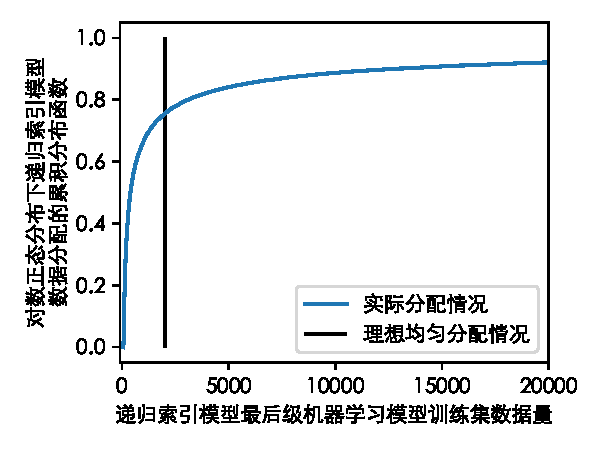
\includegraphics{figure/dispatch.pdf}
  \bicaption[{\rmi}数据分配均匀程度示意图]
    {{\rmi}数据分配均匀程度示意图}
    {The illustration of RMI data dispatch evenness}
  \label{fig:rmi-dispatch}
\end{figure}

事实上,{\li}性能对实时访问模式非常敏感。
一方面,正如上文所提到,{\rmi}的训练与推断所用到的均匀分配策略并不是最优的分配策略,会导致在{\skewacc}下呈现出次优(suboptimal)的性能表现。
另一方面,因为{\rmi}所拟合的{\cdf}结果是具有一定误差的,根据拟合出来的{\cdf}进行数据分配并不能够真正做到均匀的数据分配。
为展示这一效应,我们对{\rmi}在对数正态分布(log-normal distribution)的数据集下的数据分配情况进行了探究。
我们使用与原论文相同的{\rmi}架构,即两级{\rmi},每一级均使用{\lr}对数据进行拟合,且第二级包含1万个{\model}。
如图\ref{fig:rmi-dispatch}所示,在对数正态分布下,{\model}所分配的数据量并非维持在期望的平均数据量水平,而是具有较大的差异的。
造成这一现象的原因是{\model}对真实{\cdf}拟合所产生的误差,这是{\model}的自然特性之一{------}尽管{\model}在空间与执行时间上可以有较好的性能,但{\model}无法保证其拟合(预测)结果的正确性。
因此{\rmi}的性能在{\skewacc}下可能有较大的性能差异。

% \textbf{First, the query performance is sensitive to the runtime query distribution.}

\begin{figure}[!ht]
  \centering
  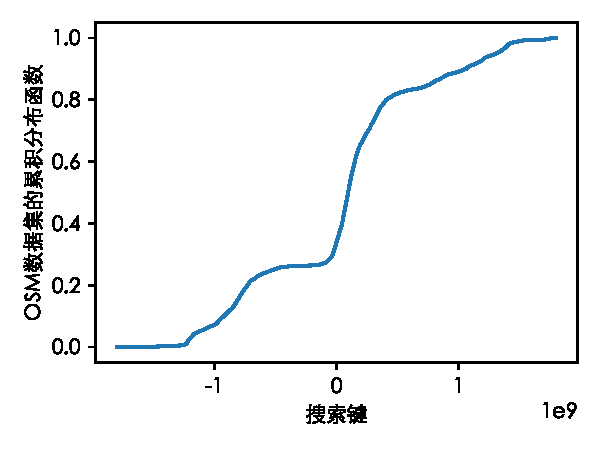
\includegraphics{figure/osm-cdf.pdf}
  \bicaption[{\osm}的{\cdf}]
    {{\osm}的{\cdf}}
    {The CDF of OSM dataset}
  \label{fig:osm-cdf}
\end{figure}

为了探究访问模式对{\li}性能的影响,我们构建了2种工作负载{------}{\uniwl}和{\skewwl}。
其中,{\uniwl}均匀随机地读取所有的搜索键,{\skewwl}则大量地访问少部分地键{------}95\%的访问发生在5\%的热键中,且这些热键存放在不同的范围内。
根据上文分析,不同的{\skewacc}对{\rmi}有不同的性能影响,而且完全取决于{\model}在训练过程中的误差,因此我们设计了多组{\skewwl}来模拟不同的{\skewacc}。
我们使用OpenStreetMap\cite{osm}(OSM)的经度数据集作为测试数据集。
OpenStreetMap是一项旨在创建一个可自由编辑的世界地图的协作项目,它最重要的产出不仅包括地图本身,而这围绕此项目产生的数据也是非常重要的产出。
OpenStreetMap被认为是当前最主要的自愿地理信息分享项目示例。
我们从OpenStreetMap中随机抽取了2亿条经度信息作为搜索键,构成{\osm}。
图\ref{fig:osm-cdf}展示了{\osm}的{\cdf}。

% We build two types of workload, uniform and skewed.
% The uniform workload evenly read every key in random order.
% Skewed workloads all have 95\% queries reading 5\% hotkeys and hotkeys reside in different ranges.
% The dataset is the same as \Cref{sec:the-good}.

% OpenStreetMap (OSM) is a collaborative project to create a free editable map of the world.
% Rather than the map itself, the data generated by the project is considered its primary output.
% The creation and growth of OSM has been motivated by restrictions on use or availability of map information across much of the world, and the advent of inexpensive portable satellite navigation devices.
% [6] OSM is considered a prominent example of volunteered geographic information.

\begin{table}[!hpb]
  \centering
  \bicaption[{\li}在不同访问模式下的性能表现]
    % {一个颇为标准的三线表格\footnotemark[1]}
    {{\li}在不同访问模式下的性能表现}
    {The learned index performance under different access patterns}
  \label{tab:pattern}
  \begin{tabular}{lcccc}
    \toprule
                  & \multicolumn{4}{c}{工作负载}            \\ \cmidrule{2-5}
                  & Skewed 1 & Skewed 2 & Skewed 3 & Uniform \\ \midrule
    B树吞吐量(MOPS)           & 2.05  & 2.09  & 2.05  & 1.15  \\
    {\li}吞吐量(MOPS)           & 2.42  & 3.11  & 1.12  & 2.02  \\
    {\li}误差范围   & 14.46    & 9.57     & 21.90    & 9.95    \\ \bottomrule
  \end{tabular}
\end{table}

根据表\ref{tab:pattern},在不同访问模式下面,{\li}的性能变化较为剧烈,甚至有时会比B树还差。
比如,在第一个{\skewwl}下,{\li}的性能和B树相近,但在第三个{\skewwl}下,{\li}的性能比B树慢45.2\%。
根据上文分析,以上结果是符合预期的。
{\li}性能是由误差值决定的,每一个具体的查询键对应的性能是由最终为它进行预测的最后级{\model}的误差决定的。
同时,不同的{\model}会有不一样的误差值,因此不同的查询键会有不一样的查询性能。
因为在{\rmi}的训练过程中,{\model}可能会分配极度不均匀的数据量,因此不同{\model}对应的误差值也会有极大的差异。
表\ref{tab:pattern}的最后一行给出了最常被访问{\model}的平均误差值。
在我们的例子里,对于{\skewwl},这个平均值是5\%热键对应的{\model}的误差,对于均匀工作负载,这是所有{\model}的平均误差。
最常被访问{\model}的平均误差值在第一个{\skewwl}和第三个{\skewwl}下远高于其他例子。
综上所述,{\li}的性能在{\skewwl}甚至比B树还要糟糕。

% \Cref{tab:skewdata} shows that the \li is not always better than \bt when varying the query distribution.
% For example, under the 1st skewed workload, \li's performance is similar to \stx, and under the 3rd skewed workloads, \li is 45.2\% slower than \stx.
% This is because each query's performance is dominated by the error bound of the 2nd stage model which predicts the position of target key; meanwhile, each model may have different error bound.
% The last row of \Cref{tab:skewdata} gives the average error bound of the frequently accessed models.
% Specifically, for the skewed workload, it is the average error bound of the models predicting for 5\% hotkeys, and for uniform workload, it is the average error bound of all models.
% The error bound of frequently accessed models in 1st and 3rd workloads is much higer than the others.
% As a result, \li's performance can be even worse than \stx.

\subsubsection{动态访问模式对{\li}性能的影响}

静态访问模式指的是一种访问模式不随时间变化而变化或随时间变化而变化非常小的一种访问模式变化趋势,
而动态访问模式指的是一种访问模式随时间变化而变化的一种访问模式变化趋势。
显然,对于静态访问模式,计算机系统能够更简单轻松地规划、管理,相对动态访问模式。
然而不幸的是,在现实情况下很难找到能够被认为是静态的应用,它们的访问模式往往是动态变化的。
对于一个系统或者一个解决方案而言,真正重要的问题是,应用行为,包括访问模式在内,有多么动态。

% The access patterns of user requests may be static, so that they do not change over time, or dynamic.
% It is obviously considerably easier to plan for and manage the static environments than would be the case for dynamic distributed systems.
% Unfortunately, it is difficult to find many real-life distributed applications that would be classified as static.
% The significant question, then, is not whether a system is static or dynamic, but how dynamic it is.
% Incidentally, it is along this dimension that the relationship between the distributed database design and query processing is established.

然而,类似第\ref{sec:dist-challenge}节讨论的,{\li}的设计并没有考虑动态的访问模式。
事实上,{\li}目前是一种“一次构建不再改变”的索引结构。
因此当面对真实场景中随处可见的动态访问模式,{\li}的性能将会更加的波动剧烈且不可预测,{\li}的应用前景再一次收到严重挑战。
